\section{FLAT PLATE TEST CASE}

Schematic diagram for conjugate heat transfer test case:\\

\begin{figure}[th!]
\subfigure[Grid dependence study with normalized temperature.]{
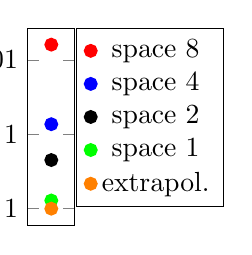
\begin{tikzpicture}[baseline,trim axis left]
\begin{axis}[ at={(0pt,0pt)}, name=plot, xlabel=  ,ylabel= T, legend pos=outer north east, width=0.6cm,scale only axis,height=2.5cm,
xtick=\empty]
\addplot[color=red, mark=*, only marks, line width=1pt] plot coordinates {
    (1,4.0879768830/4.043359014)
};
\addplot[color=blue, mark=*, only marks, line width=1pt] plot coordinates {
    (1,4.0662876068/4.043359014)
};
\addplot[color=black, mark=*, only marks, line width=1pt] plot coordinates {
    (1,4.0565397534/4.043359014)
};
\addplot[color=green, mark=*, only marks, line width=1pt] plot coordinates {
    (1,4.0455946121/4.043359014)
};
\addplot[color=orange, mark=*, only marks, line width=1pt] plot coordinates {
    (1,4.043359014/4.043359014)
};
\legend{space 8,space 4,space 2,space 1, extrapol.}
\end{axis}
\end{tikzpicture}
    \label{fig:subfig1}
}
\subfigure[Grid, space 8.]{
\includegraphics[trim=0cm 0cm 0cm 0cm, width=4cm]{figures/grid4.png}
    \label{fig:subfig2}
}
\subfigure[Flat plate.]{
\includegraphics[trim = 10mm 120mm 20mm 5mm, width=4cm]{figures/Luikov4.pdf}
    \label{fig:subfig3}
}
  \caption{Grid for computational setup.}
\end{figure}
\newpage